\documentclass[tikz,border=8pt]{standalone}
% Shared look for every TikZ diagram. Load with % Shared look for every TikZ diagram. Load with % Shared look for every TikZ diagram. Load with \input{../../tools/tikz-style.tex}
\usepackage[T1]{fontenc}
\usepackage{lmodern}
\renewcommand{\sfdefault}{lmr}  % diagrams use the same serif as the text
\usetikzlibrary{arrows.meta, positioning, shapes.geometric, calc, fit, backgrounds}
\definecolor{cblue}{HTML}{4C78A8}
\definecolor{corange}{HTML}{F58518}
\definecolor{cgreen}{HTML}{54A24B}
\definecolor{cred}{HTML}{E45756}
\definecolor{cpurple}{HTML}{B279A2}
\definecolor{cgrey}{HTML}{6B6B6B}
\tikzset{
  every picture/.style={font=\sffamily, line width=1.2pt},
  box/.style={draw=#1, fill=#1!12, rounded corners=4pt, align=center, inner sep=7pt, minimum height=1.1cm},
  box/.default=cgrey,
  arrow/.style={-{Stealth[length=3mm]}, draw=cgrey, line width=1.4pt},
  title/.style={font=\sffamily\bfseries\Large},
  note/.style={font=\sffamily\small, text=cgrey, align=center},
}
\AtBeginDocument{\hyphenpenalty=10000 \exhyphenpenalty=10000}

\usepackage[T1]{fontenc}
\usepackage{lmodern}
\renewcommand{\sfdefault}{lmr}  % diagrams use the same serif as the text
\usetikzlibrary{arrows.meta, positioning, shapes.geometric, calc, fit, backgrounds}
\definecolor{cblue}{HTML}{4C78A8}
\definecolor{corange}{HTML}{F58518}
\definecolor{cgreen}{HTML}{54A24B}
\definecolor{cred}{HTML}{E45756}
\definecolor{cpurple}{HTML}{B279A2}
\definecolor{cgrey}{HTML}{6B6B6B}
\tikzset{
  every picture/.style={font=\sffamily, line width=1.2pt},
  box/.style={draw=#1, fill=#1!12, rounded corners=4pt, align=center, inner sep=7pt, minimum height=1.1cm},
  box/.default=cgrey,
  arrow/.style={-{Stealth[length=3mm]}, draw=cgrey, line width=1.4pt},
  title/.style={font=\sffamily\bfseries\Large},
  note/.style={font=\sffamily\small, text=cgrey, align=center},
}
\AtBeginDocument{\hyphenpenalty=10000 \exhyphenpenalty=10000}

\usepackage[T1]{fontenc}
\usepackage{lmodern}
\renewcommand{\sfdefault}{lmr}  % diagrams use the same serif as the text
\usetikzlibrary{arrows.meta, positioning, shapes.geometric, calc, fit, backgrounds}
\definecolor{cblue}{HTML}{4C78A8}
\definecolor{corange}{HTML}{F58518}
\definecolor{cgreen}{HTML}{54A24B}
\definecolor{cred}{HTML}{E45756}
\definecolor{cpurple}{HTML}{B279A2}
\definecolor{cgrey}{HTML}{6B6B6B}
\tikzset{
  every picture/.style={font=\sffamily, line width=1.2pt},
  box/.style={draw=#1, fill=#1!12, rounded corners=4pt, align=center, inner sep=7pt, minimum height=1.1cm},
  box/.default=cgrey,
  arrow/.style={-{Stealth[length=3mm]}, draw=cgrey, line width=1.4pt},
  title/.style={font=\sffamily\bfseries\Large},
  note/.style={font=\sffamily\small, text=cgrey, align=center},
}
\AtBeginDocument{\hyphenpenalty=10000 \exhyphenpenalty=10000}

\begin{document}
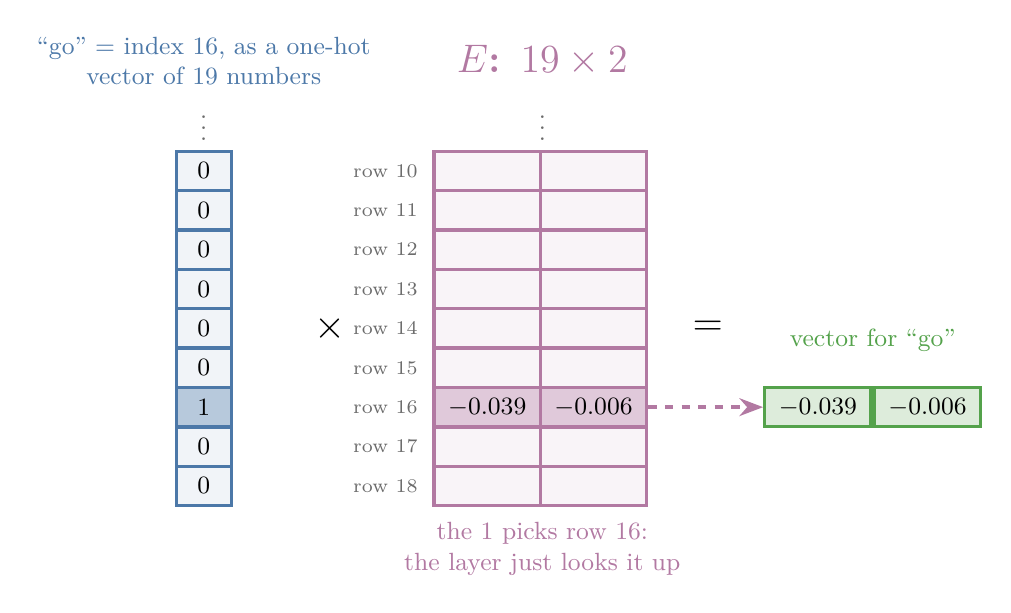
\begin{tikzpicture}
  \node[note, text=cblue] at (0,3.6) {``go'' = index 16, as a one-hot\\vector of 19 numbers};
  \node[title, text=cpurple] at (4.3,3.6) {$E$: $19 \times 2$};
  \node[font=\small, text=cgrey] at (0,2.85) {$\vdots$};
  \node[font=\small, text=cgrey] at (4.3,2.85) {$\vdots$};
  \foreach \i in {0,...,8} {
    \pgfmathtruncatemacro\r{10+\i}
    \node[draw=cblue, fill=cblue!8, minimum width=0.7cm, minimum height=0.5cm, font=\small] (o\i) at (0,2.2-0.5*\i) {0};
    \node[draw=cpurple, fill=cpurple!8, minimum width=1.35cm, minimum height=0.5cm] (a\i) at (3.6,2.2-0.5*\i) {};
    \node[draw=cpurple, fill=cpurple!8, minimum width=1.35cm, minimum height=0.5cm] (b\i) at (4.95,2.2-0.5*\i) {};
    \node[font=\scriptsize, text=cgrey, left=0.05cm of a\i] {row \r};
  }
  \node[draw=cblue, fill=cblue!40, minimum width=0.7cm, minimum height=0.5cm, font=\small] at (o6) {1};
  \node[draw=cpurple, fill=cpurple!40, minimum width=1.35cm, minimum height=0.5cm, font=\small] at (a6) {$-0.039$};
  \node[draw=cpurple, fill=cpurple!40, minimum width=1.35cm, minimum height=0.5cm, font=\small] at (b6) {$-0.006$};
  \node[font=\Large] at (1.6,0.2) {$\times$};
  \node[font=\Large] at (6.4,0.2) {$=$};
  \node[draw=cgreen, fill=cgreen!20, minimum width=1.35cm, minimum height=0.5cm, font=\small] (r1) at (7.8,-0.8) {$-0.039$};
  \node[draw=cgreen, fill=cgreen!20, minimum width=1.35cm, minimum height=0.5cm, font=\small, right=0pt of r1] (r2) {$-0.006$};
  \node[note, text=cgreen, above=0.3cm of r1.north east] {vector for ``go''};
  \draw[arrow, draw=cpurple, dashed] (b6.east) -- (r1.west);
  \node[note, text=cpurple] at (4.3,-2.6) {the 1 picks row 16:\\the layer just looks it up};
\end{tikzpicture}
\end{document}
